\documentclass[11pt]{memoir} % Maybe use Tufte ?
\usepackage[utf8]{inputenc}
\usepackage{amsmath,amsfonts,amssymb,wasysym}
\usepackage{media9, graphicx, wrapfig}
\usepackage{caption}
\usepackage{graphics,epsfig}
\usepackage{tabularx}	
\usepackage{subcaption}
\usepackage{mathrsfs}
\usepackage{listings}
%\usepackage{xcolor}
\usepackage[usenames, dvipsnames]{color}
\usepackage{pgf}
\usepackage{appendix}
\usepackage{etoolbox}
\usepackage{booktabs}
\usepackage{gensymb}
\usepackage{verse}
\usepackage{adjustbox}
\usepackage{array}	 
\usepackage{todonotes}
\usepackage{marginnote}
\usepackage{lscape}
\usepackage{float}


\setlength{\parindent}{2em}

\setlength{\parskip}{.2em}


\newenvironment{rotatepage}%
{\clearpage\pagebreak[4]\global\pdfpageattr\expandafter{\the\pdfpageattr/Rotate 90}}%
{\clearpage\pagebreak[4]\global\pdfpageattr\expandafter{\the\pdfpageattr/Rotate 0}}%


\definecolor{codegreen}{rgb}{0,0.6,0}
\definecolor{codegray}{rgb}{0.5,0.5,0.5}
\definecolor{codepurple}{rgb}{0.58,0,0.82}
\definecolor{backcolour}{rgb}{0.95,0.95,0.92}

\lstdefinestyle{mystyle}{
	backgroundcolor=\color{backcolour},   
	commentstyle=\color{codegreen},
	keywordstyle=\color{magenta},
	numberstyle=\tiny\color{codegray},
	stringstyle=\color{codepurple},
	basicstyle=\ttfamily\footnotesize,
	breakatwhitespace=false,         
	breaklines=true,                 
	captionpos=b,                    
	keepspaces=true,                 
	numbers=left,                    
	numbersep=5pt,                  
	showspaces=false,                
	showstringspaces=false,
	showtabs=false,                  
	tabsize=2
}

\lstset{style=mystyle}
%\lstset{inputpath=../CodeForListings/}


\usepackage{tikz}
\usetikzlibrary{shapes.geometric, arrows}
\tikzstyle{startstop} = [rectangle, rounded corners, minimum width=3cm, minimum height=1cm,text centered, draw=black, fill=red!30]
\tikzstyle{io} = [trapezium, trapezium left angle=75, trapezium right angle=105, minimum width=1.5cm, minimum height=1cm, text centered, draw=black, fill=blue!30]
\tikzstyle{process} = [rectangle, minimum width=3cm, minimum height=1cm, text centered, draw=black, fill=orange!30]
\tikzstyle{decision} = [rectangle,, rounded corners, minimum width=2cm, minimum height=1cm, text centered, draw=black, fill=green!30]
\tikzstyle{arrow} = [thick,->,>=stealth]


\newcommand{\attrib}[1]{%
\nopagebreak{\raggedleft\footnotesize #1\par}}
\renewcommand{\poemtitlefont}{\normalfont\large\itshape\centering}


\captionsetup[subsub]{font=footnotesize,labelfont={bf,sf}}
\setsecnumdepth{subsubsection}
\settocdepth{subsubsection}



\BeforeBeginEnvironment{appendices}{\clearpage}

\usepackage{subfiles}
\graphicspath{{../Figures/}{../../Figures/}}





\title{\textbf{Laki To Tambora} \\ A study of ice cores}
\author{Thea Quistgaard}
\date{Master Thesis 2020/2021}

\begin{document}
\lstset{language=python}
\frontmatter

\maketitle

\begin{figure}[h]
	\centering
	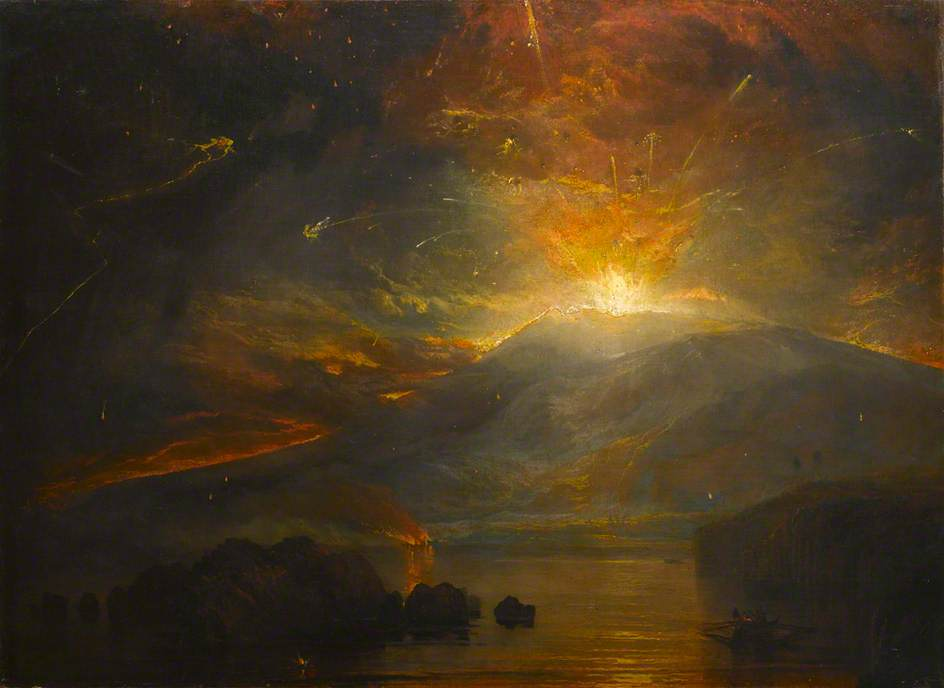
\includegraphics[width=0.8\textwidth]{TurnerEruptionofSoufriere-Mountains.jpg}
	\caption{J. M. W. Turner: \textit{The Eruption of the Soufriere Mountains}}
	\label{Fig:Turner}
\end{figure}


\newpage


\poemtitle{Darkness}
\settowidth{\versewidth}{Rayless, and pathless, and the icy earth}
\begin{verse}[\versewidth]
	I had a dream, which was not all a dream.\\
	The bright sun was extinguish'd, and the stars\\
	Did wander darkling in the eternal space,\\
	Rayless, and pathless, and the icy earth\\
	Swung blind and blackening in the moonless air;\\
	Morn came and went—and came, and brought no day.
\end{verse}
\attrib{Lord Byron (1788--1824)}


\section{Acknowledgments}


\newpage
\section{Abstract}

\newpage

\listoftodos

\tableofcontents*{}


\newpage
\listoffigures

\listoftables

\lstlistoflistings


\mainmatter

\chapter[Introduction][Introduction]{Introduction}

\subfile{../Chapters/Introduction/Chapter_Introduction2}


\chapter[Ice Theory][Ice Theory]{The theory of ice cores}

\subfile{../Chapters/IceTheory/Chapter_IceTheory2}


\chapter[Data][Data]{Isotopic Data: Laki to Tambora as seen in N Ice Cores.}

\subfile{../Chapters/Data/Chapter_Data2}



\chapter[Signal Analysis \& Comp. Meth.][Signal Analysis \& Comp. Meth.]{Signal Analysis and Computational Methods}

\subfile{../Chapters/SignalAnalysis/Chapter_SignalAnalysisAndCompMeth}


%\chapter[Computational Methods]{Computational Methods}

%\subfile{../Chapters/ComputationalMethods/Chapter_ComputationalMethods2}


\chapter[Method][Method]{Estimating $\sigma$ from Data: Methods and Algorithms}

\subfile{../Chapters/Method/Chapter_Method2}


\chapter[Results]{Results}
\subfile{../Chapters/Results/Chapter_Results2}


%\chapter[Temperature Reconstruction]{Temperature Reconstruction}

%\subfile{../Chapters/TemperatureReconstruction/Chapter_TemperatureReconstruction2}


%\chapter[Layer Counting][Layer Counting]{Layer Counting and Annual Layer Thickness Estimation}

%\subfile{../Chapters/LayerCounting/Chapter_LayerCounting2}



\chapter[Conclusion][Conclusion]{Conclusion}

\subfile{../Chapters/Conclusion/Chapter_Conclusion2}


\backmatter

\bibliographystyle{plain} 
\bibliography{/home/thea/Documents/Bibliographies/MasterThesis.bib}

%https://reader.elsevier.com/reader/sd/pii/S0039914019305375?token=2655091B0658E162E9C8C95D1AB1B21B2289F565CA3596158B63639417D66BEFC3345B6AD8E27A8453C968554CEDE2CB

%https://pubs.acs.org/doi/pdf/10.1021/acs.analchem.9b04811
\appendix 
\addcontentsline{toc}{chapter}{APPENDICES}

\chapter[Appendices][Appendices]{Appendices}
\subfile{../Chapters/Appendix/Chapter_Appendix2}
	
\end{document}